\documentclass[conference]{IEEEtran}
\IEEEoverridecommandlockouts
% Template version as of 6/27/2024

\usepackage{cite}
\usepackage{amsmath,amssymb,amsfonts}
\usepackage{algorithmic}
\usepackage{graphicx}
\usepackage{textcomp}
\usepackage{xcolor}
\usepackage{booktabs}
\usepackage{array}
\usepackage{url}

\def\BibTeX{{\rm B\kern-.05em{\sc i\kern-.025em b}\kern-.08em
    T\kern-.1667em\lower.7ex\hbox{E}\kern-.125emX}}

\begin{document}

\title{A Comparison of Attention-Based and Attention-Free Object Detection Architectures for Motorcyclist Helmet-Use Detection}

\author{
\IEEEauthorblockN{1\textsuperscript{st} Author Name}
\IEEEauthorblockA{\textit{Department Name} \\
\textit{Institution Name} \\
City, Country \\
email@example.com}
\and
\IEEEauthorblockN{2\textsuperscript{nd} Author Name}
\IEEEauthorblockA{\textit{Department Name} \\
\textit{Institution Name} \\
City, Country \\
email@example.com}
}

\maketitle

\begin{abstract}
Helmet use is the primary protective factor for motorcyclists, and automatic compliance detection from traffic cameras can support road-safety enforcement. Attention mechanisms now dominate computer vision, yet their benefit for helmet detection on small datasets remains under-examined. This study compares four object-detection architectures across the attention spectrum: YOLOv8s as a pure CNN, YOLO11s with partial attention through C2PSA blocks, RT-DETR-l as a full-attention transformer, and YOLOv8s augmented with CBAM. All models were trained on a public dataset of 1,803 images covering helmet, license plate, and motorcyclist classes. The training protocol was identical and included COCO transfer learning, 1280 pixel resolution, and matched augmentation. Each model was evaluated on a held-out test split with multiple seeds, and paired t-tests assessed differences. Under this protocol, no attention variant surpassed the plain YOLOv8s. The baseline achieved the highest mAP@0.5 of $0.9592 \pm 0.0014$ at approximately 296 FPS. Adding CBAM significantly reduced mAP@0.5 by $0.0113$ ($t(2) = 10.9$, $p = 0.008$, Cohen's $d \approx 9.1$). YOLO11s and RT-DETR-l did not differ significantly from the baseline. Because the baseline approaches the ceiling and the number of seeds is small, the equivalence claims represent an absence of evidence rather than evidence of absence. Within this scope, the added complexity of attention does not pay off.
\end{abstract}

\begin{IEEEkeywords}
helmet detection, object detection, attention mechanism, YOLO, RT-DETR, CBAM, motorcycle safety
\end{IEEEkeywords}

\section{Introduction}
Motorcycles account for a large share of traffic-accident casualties, especially in countries where they dominate daily mobility, and the helmet is the most decisive protective factor against fatal head injuries. Manual observation of helmet compliance does not scale to real traffic volumes, while automatic object detection from camera footage can operate continuously and consistently \cite{ref1}.

Object detection has shifted over the past decade from accurate but slow two-stage approaches to fast single-stage detectors, with the YOLO family becoming the de facto standard for real-time applications \cite{ref5, ref_terven}. In parallel, attention mechanisms emerged from the Transformer \cite{ref10} and were adapted to images through the Vision Transformer \cite{ref11}. Transformer-based detectors such as DETR \cite{ref8} and its real-time descendant RT-DETR \cite{ref7} now compete directly with CNNs, and lightweight attention modules such as Squeeze-and-Excitation \cite{ref12} and CBAM \cite{ref9} are popular ways to inject attention into existing CNN backbones.

The trend of adding attention to helmet-detection models has produced a number of positive reports. Several recent studies inject attention modules into YOLO-family detectors and report accuracy improvements on their respective helmet datasets. However, these studies generally compare a single configuration without repetition across seeds, use protocols tuned per model, and omit statistical significance testing. The reported gains could therefore stem from hyperparameters, augmentation, or initialisation luck, rather than from the attention mechanism itself.

This study addresses that gap with a single focused research question. \textbf{Can the improvements reported by attention-based studies on helmet detection be replicated in a controlled comparison that uses a unified protocol, repetition across seeds, and significance testing?} The contributions are threefold. First, we present a controlled comparison of four detection architectures with identical hyperparameters, data, and augmentation, so that performance differences can be attributed to architectural factors. Second, we conduct a multi-seed evaluation that reports paired t-tests, Cohen's $d$ effect size, and 95\% confidence intervals, so the conclusions do not rest on the luck of a single initialisation. Third, we present a structured rebuttal of the assumption that adding attention always helps, since under our protocol no attention mechanism surpassed the pure CNN and CBAM significantly reduced accuracy.

\section{Literature Review}

\subsection{Helmet Detection}
Research on helmet detection has evolved from simple classification toward pipelines that detect, track, and classify motorcycles together with their riders. Siebert and Lin \cite{ref1} demonstrated large-scale helmet-use detection from traffic video using a single-stage detector and released a widely used annotated dataset. Benchmark challenges such as the AI City Challenge 2023 Track 5 \cite{ref3} have driven progress on multi-class helmet-violation detection under heavy class imbalance. In the enforcement context, several pipelines combine helmet detection with license-plate localisation and recognition to identify violators \cite{ref4}.

A growing body of work integrates attention mechanisms into helmet-detection models. Common patterns include adding channel-spatial attention modules to YOLO-family detectors and inserting feature-fusion blocks together with attention layers. These studies typically report accuracy improvements over their respective baselines. However, they generally compare a single configuration without repetition across seeds, use protocols tuned per model, and omit statistical significance testing. The reported gains could therefore stem from hyperparameters, augmentation, or initialisation luck, rather than from the attention mechanism itself. This methodological gap directly motivates the controlled, multi-seed comparison presented in this study.

\subsection{Object Detection Architectures and Attention}
Single-stage detectors formulate detection as direct regression of bounding boxes and classes in a single network pass, trading some accuracy for high speed \cite{ref5}. The YOLO family has become the de facto standard for real-time detection, with each iteration improving the backbone, neck, and label-assignment strategy \cite{ref_terven}. YOLOv8 represents a mature CNN generation without explicit attention modules. YOLO11 introduces positional attention blocks called C2PSA, which makes it a useful midpoint between pure CNN and transformer designs.

Attention mechanisms originated in the Transformer \cite{ref10} and were adapted to images by the Vision Transformer \cite{ref11}. In detection, DETR \cite{ref8} formulates detection as a set-prediction problem with an encoder-decoder transformer, and its real-time descendant RT-DETR \cite{ref7} addresses the slow convergence and high cost of the original. A separate line injects attention into a CNN through lightweight modules. CBAM \cite{ref9} sequentially combines channel attention and spatial attention to emphasise both what is important and where it appears. Surveys of attention in vision \cite{ref17, ref18} note that the effectiveness of these mechanisms depends heavily on training-data volume and task complexity. For small-object detection in particular, Cheng et al. \cite{ref23} observe that small objects within wide frames such as helmets and license plates require multi-scale features and high input resolution.

\section{Methodology}

\subsection{Dataset}
We use a public helmet-detection dataset from Roboflow Universe (NCKH 2023 Helmet Detection Project, version 19, MIT license). The dataset contains 1,803 annotated images in YOLO format with three classes: helmet, license plate, and motorcyclist. A fixed split of 1,563 training, 140 validation, and 100 test images was used throughout, and all final metrics were computed on the test split, which was never seen during training.

\subsection{Architectures Compared}
Four architectures were chosen so that they occupy different points on the spectrum of attention usage, as summarised in Table~\ref{tab:architectures}: a CNN with no attention, a CNN with partial attention, a transformer with full attention, and a controlled attention intervention added to the baseline.

\begin{table*}[!t]
\caption{The four architectures and their position on the attention spectrum.}
\label{tab:architectures}
\begin{center}
\begin{tabular}{|l|l|l|c|}
\hline
\textbf{Model} & \textbf{Paradigm} & \textbf{Attention} & \textbf{Params} \\
\hline
YOLOv8s & Single-stage CNN & None (baseline) & $\sim$11.17 M \\
\hline
YOLO11s & Single-stage CNN & Partial (C2PSA) & $\sim$9.4 M \\
\hline
RT-DETR-l & Transformer & Full (self-attention) & $\sim$32 M \\
\hline
YOLOv8s+CBAM & CNN + module & Channel and spatial & $\sim$11.51 M \\
\hline
\end{tabular}
\end{center}
\end{table*}

The YOLOv8s+CBAM variant anchors the controlled attention experiment. Three CBAM modules were inserted at the outputs of the three detection scales (P3, P4, P5) just before the detection head, so the model is identical to the plain YOLOv8s except for the added attention. The addition raises the parameter count from 11.17 to 11.51 million, an increase of about three percent. RT-DETR-l (about 32 million parameters) is far larger than the YOLO-s variants (9 to 11 million), so the comparison mixes architectural paradigm with model capacity. This is acknowledged in Section~V and discussed as a limitation.

\subsection{Training Protocol}
All models were trained with an identical protocol using the Ultralytics framework \cite{ref6} on PyTorch and a single NVIDIA RTX 4090 GPU. Each model was initialised with COCO-pretrained weights \cite{ref14}. For the CBAM variant, the attention layers were randomly initialised while the rest inherited COCO weights. The configuration used 1280-pixel input resolution (chosen because helmets and license plates occupy small regions), automatic batch-size, automatic optimiser, and identical augmentation (mosaic, HSV shifting, horizontal flipping). Early stopping used patience 25 over a maximum of 100 epochs.

Reproducibility was enforced by fixing seeds for \texttt{random}, NumPy, and PyTorch with cuDNN in deterministic mode. Each run saved its configuration and environment details. Each model was retrained on three seeds (42, 0, 1), except RT-DETR-l, which was run on two seeds because its training cost is far higher (about 190 minutes per run versus about 26 minutes for the YOLO variants).

\subsection{Evaluation Metrics and Statistical Testing}
The primary metrics are mAP@0.5 and mAP@[.5:.95], following object-detection convention, supplemented by inference speed in frames per second (FPS). FPS was measured on a single run while the GPU was idle (no other processes running) using the Ultralytics built-in benchmark on the full test split, on the same hardware (NVIDIA RTX 4090, batch size 1) for all models. The figures are estimates at a single hardware point and will differ on other configurations.

To assess the significance of accuracy differences, we paired the results between models on the same seed and applied a paired t-test to the mAP@0.5 difference of each seed pair, with $\alpha = 0.05$. We also report Cohen's $d$ effect size and the 95\% confidence interval for the mean difference. Pairing by seed controls for initialisation variation. This protocol follows recent guidance on accounting for variance in machine learning benchmarks, which argues that single-run comparisons are unreliable \cite{ref_bouthillier}. With $n = 3$ for the YOLO variants and $n = 2$ for RT-DETR-l, the test is indicative: it can confirm consistent differences, but its power to reject equivalence is low.

\section{Results}

Table~\ref{tab:overall} summarises the performance of the four architectures on the test split. YOLOv8s achieved the highest mAP@0.5 together with the best inference speed. YOLO11s and RT-DETR-l were comparable in accuracy but slower. YOLOv8s+CBAM was in fact the lowest on mAP@0.5.

\begin{table*}[!t]
\caption{Performance comparison on the test split (mean $\pm$ standard deviation).}
\label{tab:overall}
\begin{center}
\begin{tabular}{|l|c|c|c|c|}
\hline
\textbf{Model} & \textbf{$n$} & \textbf{mAP@0.5} & \textbf{mAP@[.5:.95]} & \textbf{FPS} \\
\hline
\textbf{YOLOv8s} & 3 & $\mathbf{0.9592 \pm 0.0014}$ & $0.6862 \pm 0.0046$ & $\mathbf{\sim 296}$ \\
\hline
YOLO11s & 3 & $0.9569 \pm 0.0046$ & $\mathbf{0.6898 \pm 0.0030}$ & $\sim 189$ \\
\hline
RT-DETR-l & 2 & $0.9588 \pm 0.0151$ & $0.6764 \pm 0.0205$ & $\sim 55$ \\
\hline
YOLOv8s+CBAM & 3 & $0.9479 \pm 0.0004$ & $0.6810 \pm 0.0045$ & $\sim 290$ \\
\hline
\end{tabular}
\end{center}
\end{table*}

\subsection{Effect of the Attention Mechanism}
The main axis of the study is the presence and type of attention. Under a training protocol arranged for YOLO, this axis shows no advantage from attention. Fig.~\ref{fig:attention} visualises the mAP@0.5 of the four models together with the standard deviation across seeds. YOLOv8s without attention leads.

\begin{figure}[htbp]
\centerline{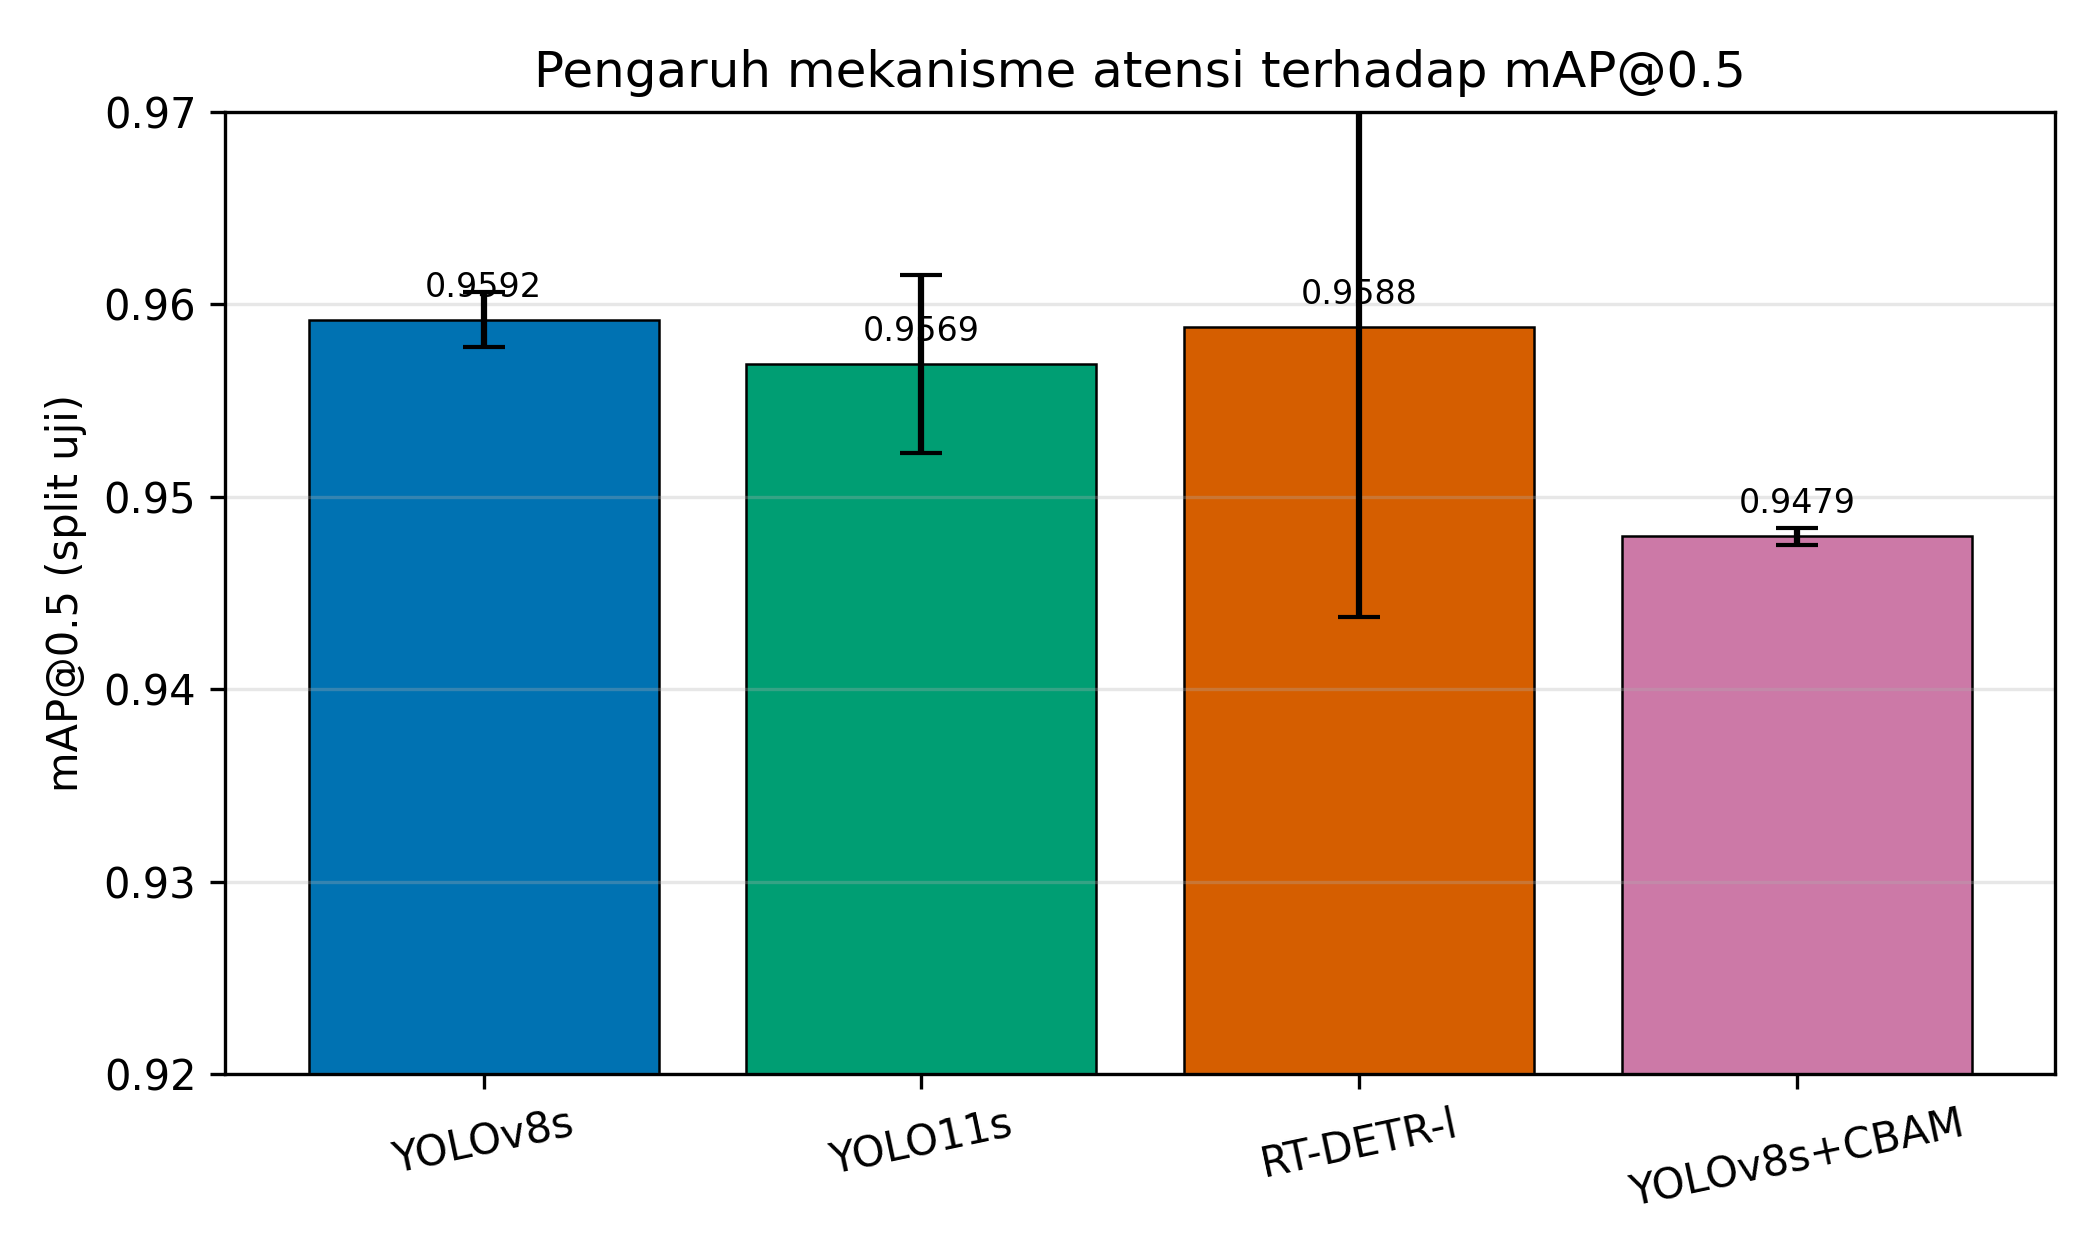
\includegraphics[width=0.95\columnwidth]{../results/figures/fig1_attention_mAP50.png}}
\caption{Effect of the attention mechanism on mAP@0.5 on the test split. Error bars show the standard deviation across seeds. No attention-based variant surpasses YOLOv8s, and CBAM is in fact the lowest.}
\label{fig:attention}
\end{figure}

\begin{table*}[!t]
\caption{Paired t-test results for the mAP@0.5 difference.}
\label{tab:ttest}
\begin{center}
\begin{tabular}{|l|c|c|c|c|c|}
\hline
\textbf{Comparison} & \textbf{$\Delta$} & \textbf{$t$(df)} & \textbf{$p$} & \textbf{$d$} & \textbf{95\% CI} \\
\hline
YOLOv8s vs YOLO11s & $+0.0023$ & $0.73$ (2) & $0.54$ & $0.61$ & $[-0.011, +0.016]$ \\
\hline
YOLOv8s vs RT-DETR-l & $+0.0004$ & $0.11$ (1) & $0.93$ & n/a & $[-0.140, +0.142]$ \\
\hline
YOLOv8s vs CBAM & $+0.0113$ & $10.9$ (2) & $0.008$ & $9.1$ & $[0.0068, 0.0157]$ \\
\hline
\end{tabular}
\end{center}
\end{table*}

Table~\ref{tab:ttest} reports the paired t-tests. Two patterns emerge. First, neither YOLO11s nor RT-DETR-l differs significantly from the baseline. The Cohen's $d$ for YOLO11s indicates a medium effect by convention, but the $n = 3$ design lacks the power to reach significance. The very wide confidence interval for RT-DETR-l reflects an unstable estimate from only two seeds with far-apart results ($0.9482$ and $0.9695$), so the equivalence claim is better described as an absence of evidence rather than evidence of equivalence. Second, adding the CBAM module reduced mAP@0.5 with high statistical significance and a very large effect size. The small standard deviations of the baseline and the CBAM variant confirm that the reduction is stable across initialisations. This result holds under a YOLO-tuned protocol and shows that inserting CBAM is detrimental \emph{under those conditions}, not that attention is universally detrimental.

\subsection{Per-Class Performance}
On the YOLOv8s baseline, per-class accuracy tracks object size and distinctiveness, as shown in Fig.~\ref{fig:perclass}. The motorcyclist class is the easiest because the rider is large and prominent. The license plate class follows, helped by its distinctive rectangular shape. The helmet class is the most challenging because helmets are small, easily confused with other head accessories such as caps or hair, and varied in colour and viewing angle. The helmet class is also the most relevant to the application, so it is the main determinant of remaining room for improvement.

\begin{figure}[htbp]
\centerline{
\includegraphics[width=0.95\columnwidth]{../results/figures/fig2_per_class.png}}
\caption{Per-class performance of YOLOv8s on the test split. The helmet class is the most challenging because of its small size and visual ambiguity.}
\label{fig:perclass}
\end{figure}

\subsection{Speed Trade-Off}
The speed difference is far larger than the accuracy difference, as shown in Fig.~\ref{fig:speed}. RT-DETR-l runs at about 55 FPS, roughly five times slower than YOLOv8s at about 296 FPS, and demands about 190 minutes per training run compared with about 26 minutes for the YOLO variants. YOLO11s sits in the middle at about 189 FPS. The CBAM variant is nearly as fast as the baseline because the added module is lightweight. When accuracy is practically equal across the four models, the computational cost of the transformer does not pay off on this task. Fig.~\ref{fig:speed} places YOLOv8s in the most advantageous corner because it leads on both axes simultaneously.

\begin{figure}[htbp]
\centerline{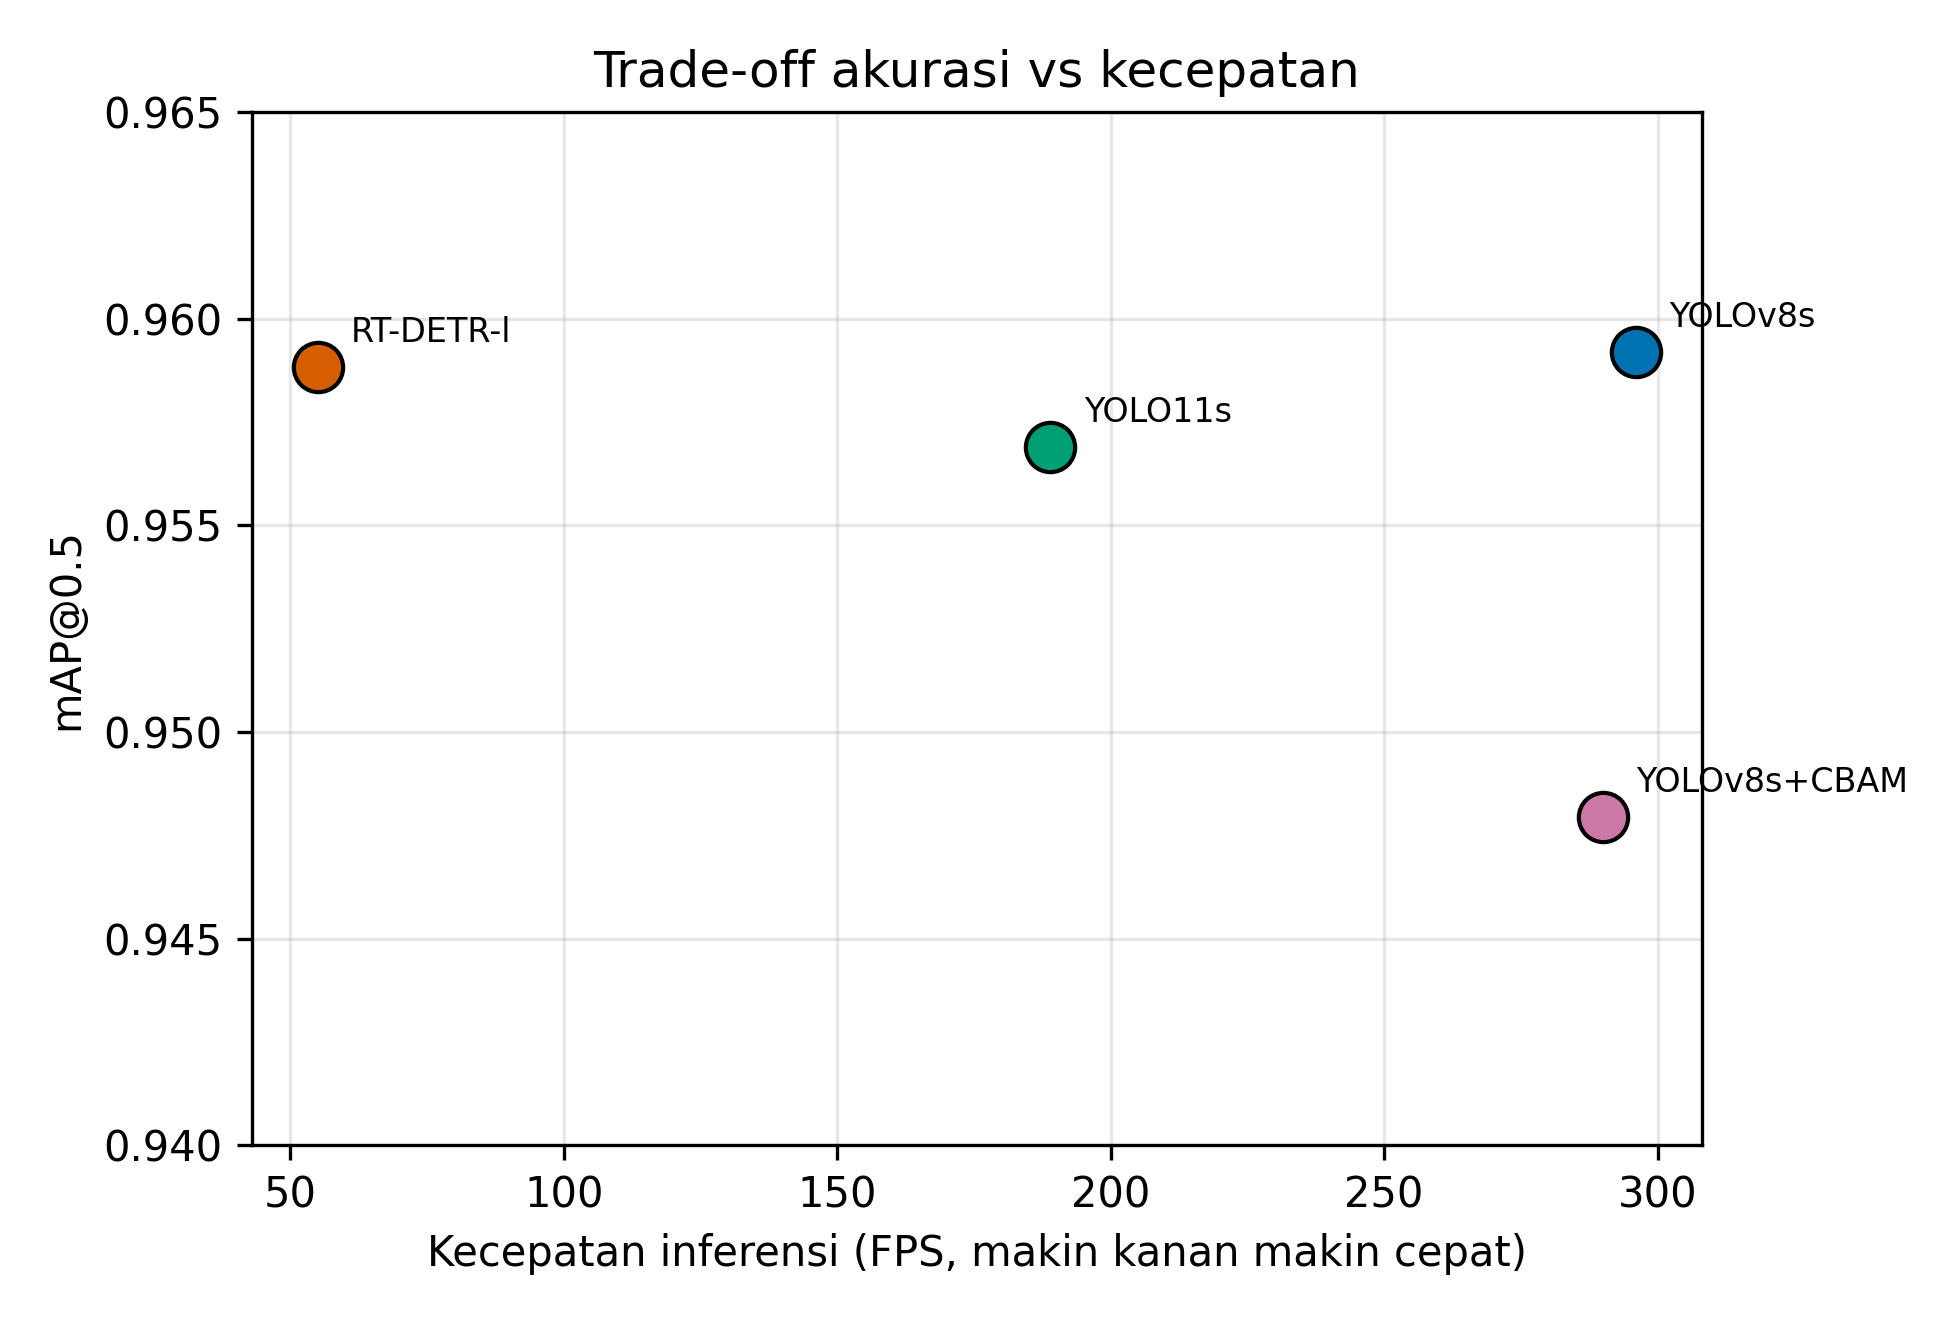
\includegraphics[width=0.95\columnwidth]{../results/figures/fig3_accuracy_speed.png}}
\caption{Accuracy (mAP@0.5) versus speed (FPS) trade-off. YOLOv8s occupies the most advantageous position because it leads on both axes simultaneously.}
\label{fig:speed}
\end{figure}

\subsection{Qualitative Analysis}
Fig.~\ref{fig:qualitative} shows a typical YOLOv8s detection output on a test image, where the rider, the helmet, and the license plate are detected simultaneously with tight bounding boxes. Visual inspection of the test sample shows that remaining errors tend to appear on very small or partially occluded helmets, consistent with the quantitative finding that the helmet class is the most difficult.

\begin{figure}[htbp]
\centerline{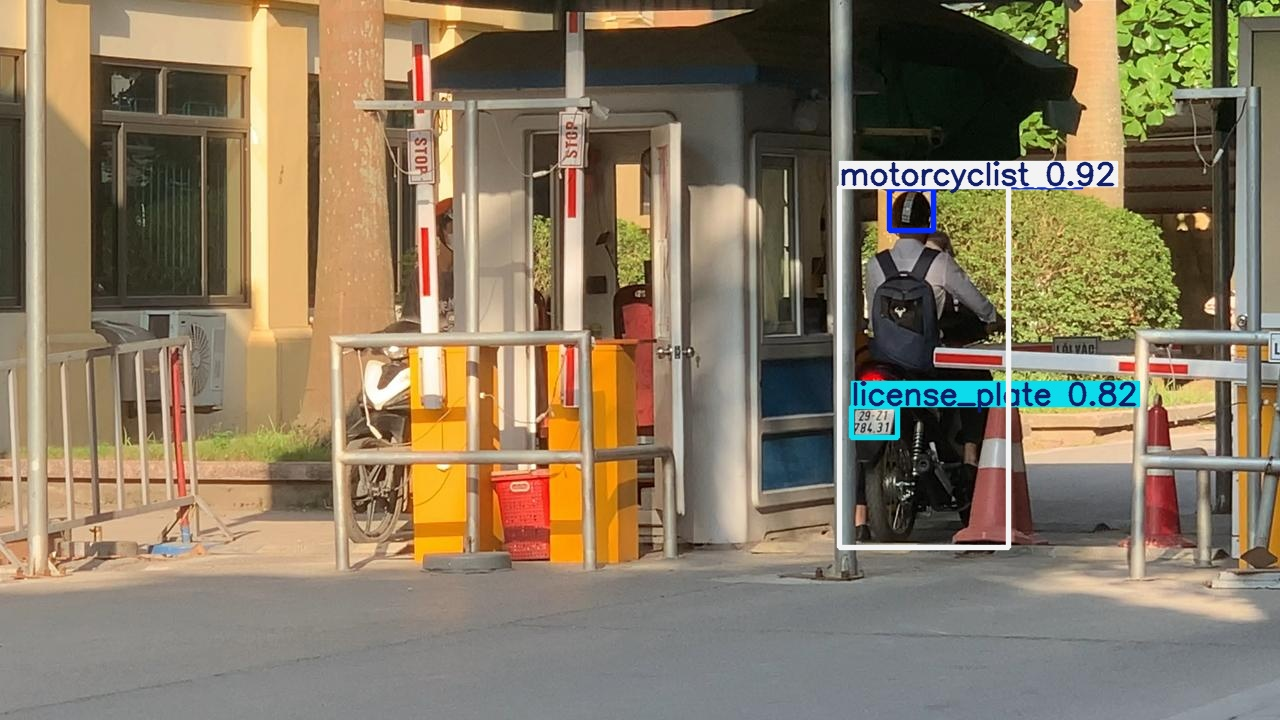
\includegraphics[width=0.95\columnwidth]{../results/figures/fig4_detection_example.png}}
\caption{Example of YOLOv8s detection output on a test image. The rider, the helmet, and the license plate are all detected simultaneously.}
\label{fig:qualitative}
\end{figure}

\section{Discussion}

The central finding of this study runs counter to the common intuition that adding attention helps. Under a YOLO-tuned protocol on a small, relatively easy dataset, no attention mechanism surpassed the pure-CNN YOLOv8s, and CBAM was even significantly detrimental. We discuss why this happens, an important rival hypothesis, and the scope of the claim.

\subsection{Why Attention Does Not Help in This Setting}
The training set contains only 1,563 images, and the baseline already reaches about $0.96$ mAP@0.5. Almost no headroom remains for a more complex mechanism to demonstrate an advantage. Attention mechanisms are also data-hungry and benefit most from large-scale pretraining \cite{ref17, ref18}. In the small-data regime, the theoretical advantage of attention does not materialise and the model bears the cost of unused capacity.

The CBAM result has an additional explanation. The CBAM modules are randomly initialised while the rest of the network inherits COCO weights. The fresh modules disrupt the mature feature flow obtained from transfer learning, and with limited data there is not enough gradient signal to recover from this disruption. The result is a small but consistent reduction that is stable across seeds. Complexity is also not free in operational terms. RT-DETR-l is roughly five times slower than YOLOv8s while showing no mAP reward, and CBAM adds a computational path at every detection scale. When accuracy is practically equal, the additional cost of attention does not pay off.

\subsection{A Rival Hypothesis for the CBAM Reduction}
The CBAM reduction does not automatically imply that CBAM is useless for helmet detection. Several design factors can plausibly explain it. The module placement at the detection head, rather than in the backbone, may be suboptimal. The fresh layers may disrupt pretrained weights more than additional epochs can recover. The learning rate was not tuned separately for the attention parameters. A systematic ablation that varies placement, trains from scratch, lengthens the schedule, and applies a separate learning rate for the attention module is needed to isolate the exact cause and is part of future work.

\subsection{Scope of the Claim}
This study does not conclude that attention is useless in general. Under one YOLO-tuned protocol, on one small and relatively easy dataset, and with a baseline that already approaches the ceiling, adding attention did not improve accuracy and CBAM reduced it significantly. The equivalence of YOLO11s and RT-DETR-l should be read as an absence of evidence of a difference rather than evidence of equivalence, since the ceiling effect suppresses statistical power. The plausible rival hypothesis that the attention-based models were not trained on their optimal recipe also cannot be ruled out. The practical implication, within this scope, is that a simple CNN such as YOLOv8s remains the most rational choice for real-time helmet detection on similar data.

\section{Threats to Validity}

We highlight four limitations that constrain the generalisation of these findings.

\textbf{Single small, relatively clean dataset.} The dataset is curated, well-lit, and lightly occluded, which differs from real road CCTV where heavy occlusion, nighttime lighting, rain, and high traffic density are the norm. Generalisation to such conditions, where the global context modelled by attention may genuinely help, has not been verified.

\textbf{Limited seeds and low statistical power.} The YOLO variants were evaluated with three seeds and RT-DETR-l with two. Combined with the ceiling effect at $0.96$ mAP@0.5, this leaves the paired t-test underpowered to detect small improvements. Equivalence claims for YOLO11s and RT-DETR-l therefore represent an absence of evidence rather than evidence of equivalence, and the wide $95\%$ confidence interval for RT-DETR-l ($[-0.140, +0.142]$) reflects this instability.

\textbf{Architecture-versus-capacity confounding.} RT-DETR-l contains about 32 million parameters, while the YOLO-s variants contain 9 to 11 million. The comparison therefore mixes architectural paradigm with model capacity. A size-matched control such as YOLOv8m (about 25 million parameters) would isolate the paradigm effect and is part of future work.

\textbf{YOLO-tuned hyperparameters.} Hyperparameters were unified across architectures and were not tuned per model. Transformers and attention-based models may require different learning rates, warm-up schedules, or augmentations, so the results for these models may represent a lower bound rather than their true potential.

\section{Conclusion}

We compared four object-detection architectures spanning the attention spectrum (YOLOv8s, YOLO11s, RT-DETR-l, YOLOv8s+CBAM) for motorcyclist helmet-use detection, using an identical training protocol with multi-seed evaluation and paired t-tests. Under a YOLO-tuned protocol on a small, relatively easy dataset, no attention mechanism surpassed the pure-CNN YOLOv8s, and CBAM significantly reduced accuracy. YOLOv8s also delivered the fastest inference. The equivalence of YOLO11s and RT-DETR-l is best read as an absence of evidence of a difference, given the ceiling effect and the small number of seeds. These findings are best interpreted as a practical caution against the assumption that adding attention always helps on small-scale helmet-detection tasks, not as a general verdict on attention mechanisms.

Future work follows directly from the limitations. Generalisation should be tested on larger and more challenging datasets, including real CCTV footage. Per-architecture hyperparameter tuning and size-matched comparisons (such as YOLOv8m as a control for RT-DETR-l) would isolate paradigm effects from capacity effects. A systematic CBAM ablation that varies placement, lengthens training schedules, and uses a separate learning rate for the attention parameters would clarify whether the observed reduction is intrinsic or an artefact of the experimental design.

\section*{Statements}

\textbf{Data Availability.} The dataset is publicly available through Roboflow Universe under the name NCKH 2023 Helmet Detection Project, version 19, with the MIT license. The training scripts, configurations, and experiment notebooks are available in the authors' research repository.

\textbf{Conflict of Interest.} The authors declare no conflict of interest.

\textbf{Funding.} No specific funding is reported for this study.

\section*{Acknowledgment}

The authors thank the course instructors for their guidance throughout the project. The authors also acknowledge the use of AI-based tools for assistance in experiment design, analysis, and manuscript drafting. All methodological decisions, verification of numerical results, and final responsibility for the content rest with the authors.

\begin{thebibliography}{00}

\bibitem{ref1} F. W. Siebert and H. Lin, ``Detecting motorcycle helmet use with deep learning,'' \textit{Accident Analysis \& Prevention}, vol. 134, p. 105319, 2020.

\bibitem{ref3} M. Naphade et al., ``The 7th AI City Challenge,'' in \textit{Proc. IEEE/CVF Conf. Computer Vision and Pattern Recognition Workshops (CVPRW)}, 2023.

\bibitem{ref4} W. Jia et al., ``Real-time automatic helmet detection of motorcyclists in urban traffic using improved YOLOv5 detector,'' \textit{IET Image Processing}, vol. 15, no. 14, pp. 3623--3637, 2021.

\bibitem{ref5} J. Redmon, S. Divvala, R. Girshick, and A. Farhadi, ``You only look once: Unified, real-time object detection,'' in \textit{Proc. IEEE Conf. Computer Vision and Pattern Recognition (CVPR)}, 2016, pp. 779--788.

\bibitem{ref6} G. Jocher, A. Chaurasia, and J. Qiu, ``Ultralytics YOLO,'' 2023. [Online]. Available: \url{https://github.com/ultralytics/ultralytics}

\bibitem{ref7} Y. Zhao et al., ``DETRs beat YOLOs on real-time object detection,'' in \textit{Proc. IEEE/CVF Conf. Computer Vision and Pattern Recognition (CVPR)}, 2024.

\bibitem{ref8} N. Carion, F. Massa, G. Synnaeve, N. Usunier, A. Kirillov, and S. Zagoruyko, ``End-to-end object detection with transformers,'' in \textit{Proc. European Conf. Computer Vision (ECCV)}, 2020, pp. 213--229.

\bibitem{ref9} S. Woo, J. Park, J.-Y. Lee, and I. S. Kweon, ``CBAM: Convolutional block attention module,'' in \textit{Proc. European Conf. Computer Vision (ECCV)}, 2018, pp. 3--19.

\bibitem{ref10} A. Vaswani et al., ``Attention is all you need,'' in \textit{Advances in Neural Information Processing Systems (NeurIPS)}, 2017, pp. 5998--6008.

\bibitem{ref11} A. Dosovitskiy et al., ``An image is worth 16x16 words: Transformers for image recognition at scale,'' in \textit{Proc. Int. Conf. Learning Representations (ICLR)}, 2021.

\bibitem{ref12} J. Hu, L. Shen, and G. Sun, ``Squeeze-and-excitation networks,'' in \textit{Proc. IEEE Conf. Computer Vision and Pattern Recognition (CVPR)}, 2018, pp. 7132--7141.

\bibitem{ref13} T.-Y. Lin, P. Goyal, R. Girshick, K. He, and P. Doll\'ar, ``Focal loss for dense object detection,'' in \textit{Proc. IEEE Int. Conf. Computer Vision (ICCV)}, 2017, pp. 2980--2988.

\bibitem{ref14} T.-Y. Lin et al., ``Microsoft COCO: Common objects in context,'' in \textit{Proc. European Conf. Computer Vision (ECCV)}, 2014, pp. 740--755.

\bibitem{ref15} Z. Liu et al., ``Swin Transformer: Hierarchical vision transformer using shifted windows,'' in \textit{Proc. IEEE/CVF Int. Conf. Computer Vision (ICCV)}, 2021, pp. 10012--10022.

\bibitem{ref16} Y. Li, H. Mao, R. Girshick, and K. He, ``Exploring plain vision transformer backbones for object detection,'' in \textit{Proc. European Conf. Computer Vision (ECCV)}, 2022, pp. 280--296.

\bibitem{ref17} M.-H. Guo, T.-X. Xu, J.-J. Liu, Z.-N. Liu, P.-T. Jiang, T.-J. Mu, S.-H. Zhang, R. R. Martin, M.-M. Cheng, and S.-M. Hu, ``Attention mechanisms in computer vision: A survey,'' \textit{Computational Visual Media}, vol. 8, no. 3, pp. 331--368, 2022.

\bibitem{ref18} Z. Niu, G. Zhong, and H. Yu, ``A review on the attention mechanism of deep learning,'' \textit{Neurocomputing}, vol. 452, pp. 48--62, 2021.

\bibitem{ref23} G. Cheng, X. Yuan, X. Yao, K. Yan, Q. Zeng, and J. Han, ``Towards large-scale small object detection: Survey and benchmarks,'' \textit{IEEE Trans. Pattern Anal. Mach. Intell.}, vol. 46, no. 1, pp. 521--539, 2024.

\bibitem{ref_terven} J. Terven, D.-M. C\'ordova-Esparza, and J.-A. Romero-Gonz\'alez, ``A comprehensive review of YOLO architectures in computer vision: From YOLOv1 to YOLOv8 and YOLO-NAS,'' \textit{Machine Learning and Knowledge Extraction}, vol. 5, no. 4, pp. 1680--1716, 2023.

\bibitem{ref_bouthillier} X. Bouthillier et al., ``Accounting for variance in machine learning benchmarks,'' in \textit{Proc. Machine Learning and Systems (MLSys)}, vol. 3, 2021.

\end{thebibliography}

\end{document}
